% Welcome! This is the unofficial Umeå University template.
% IMPORTANT: 
% This work, "Umeå University Unofficial Beamer Theme", is a derivative
% of "University of Udine Unofficial Beamer Theme" by Marco Basaldella, University of Udine, CC 4.0 BY. 
% (https://www.overleaf.com/latex/templates/university-of-udine-unofficial-beamer-theme/zndkgxrjsdzt) 
%
% In this derived work, changes are made to the colour scheme, title frame, selected fonts as well as 
% the images used in the title-frame and header. Otherwise, the main functionality and commands are 
% all credited to Marco Basaldella (and Till Tantau et al. for creating the beamer document class in
% the first place).  
%
% "Umeå University Unofficial Beamer Theme" is licensed under CC 4.0 by Jesper Erixon.

% See README.md for more full information about this template .

% Note that [usenames,dvipsnames] is MANDATORY due to compatibility
% issues between tikz and xcolor packages.

\documentclass[usenames,dvipsnames,10pt,aspectratio=169]{beamer} 
% Add option 'aspectratio=169' for 16:9 widescreen 
% Add option  'handout' to ignore animations
% If you have a smaller amount of text, feel free to also try '11pt'! / Jesper

\usepackage[utf8]{inputenc}
\usepackage{verbatim}
\usetheme{phd}

%%% Custom TikZ addons
\usetikzlibrary{crypto.symbols}
\usetikzlibrary{positioning}
\usetikzlibrary{keccaktree}
\tikzset{shadows=no}        % Option: add shadows to XOR, ADD, etc.\usetikzlibrary{arrows}


%%% Bibliography
\usepackage[style=authoryear,backend=biber]{biblatex}
\addbibresource{bibliography.bib}

% Author names in publication list are consistent 
% i.e. name1 surname1, name2 surname2
% See https://tex.stackexchange.com/questions/106914/biblatex-does-not-reverse-the-first-and-last-names-of-the-second-author
\DeclareNameAlias{author}{given-family}

%%% Suppress biblatex annoying warning
\usepackage{silence}
\WarningFilter{biblatex}{Patching footnotes failed}

%%% Some useful commands
% pdf-friendly newline in links
\newcommand{\pdfnewline}{\texorpdfstring{\newline}{ }} 
% Fill the vertical space in a slide (to put text at the bottom)
\newcommand{\framefill}{\vskip0pt plus 1filll}

%%% Additional packages, added by Jesper Erixon
% Use babel to neatly translate 'abstract' etc. to swedish  or other supported language
%\usepackage[swedish]{babel}

%%% Enter additional packages below (or above, I can't stop you)! / Jesper
\renewcommand{\proofname}{\sffamily{Proof}}

%%%%%%%%%%%%%%%%%%%%%%%%%%%%%%%%%%%%%%%%%%%%%%%%%%%%%%%%%%%%%%%%%%%%%%%%%%%%%%%%%%%%%
%%%%%%%%%%%%%%%%%%%%%%%%%%%%%%% YOUR PRESENTATION BELOW %%%%%%%%%%%%%%%%%%%%%%%%%%%%%
%%%%%%%%%%%%%%%%%%%%%%%%%%%%%%%%%%%%%%%%%%%%%%%%%%%%%%%%%%%%%%%%%%%%%%%%%%%%%%%%%%%%%
\title[]{A Panorama on\\Classical Cryptography}
\date[\today]{\small December 13$^{th}$, 2021}
\author[Beno\^it Viguier]{
  Beno\^it Viguier
}

\begin{document}

\begin{frame}
	\titlepage
\end{frame}

% \begin{frame}{\contentsname}
% 	\tableofcontents
% \end{frame}

% \section{Before you start}

% \begin{frame}{What is cryptography?}

% \end{frame}
\framepic[0.25]{graphics/enigma}{What is cryptography?}{
	\vspace{2cm}
	\begin{columns}
		\begin{column}{0.5\textwidth}
			\raggedleft
			
\includegraphics[width=0.5\textwidth]{graphics/imitation_game.jpg}
		\end{column}
		\begin{column}{0.5\textwidth}
			\raggedright
			
\includegraphics[width=0.5\textwidth]{graphics/A-Beautiful-Mind.jpg}
		\end{column}
	\end{columns}
}

\framepic[0.4]{graphics/computer}{What is cryptography?}{
	\vspace{4cm}
	{
		\large{\textbf{\emph{Cryptography is about communication in the presence of adversaries.}\\
				\medskip Ron Rivest}}
	}
}



\framepic[0.25]{graphics/card}{What do we want to protect?}{
	\vspace{2.75cm}
	\Large

	\begin{itemize}
		\item \emphp{Confidentiality}\medskip
		\item \lesss{Data Integrity}\medskip
		\item \lesss{Data origin authentication}\medskip
		\item \lesss{Entity authentication}\medskip
	\end{itemize}
}

\framepic[0.3]{graphics/corruption}{What do we want to protect?}{
	\vspace{2.75cm}
	\Large

	\begin{itemize}
		\item \lesss{Confidentiality}\medskip
		\item \emphp{Data Integrity}\medskip
		\item \lesss{Data origin authentication}\medskip
		\item \lesss{Entity authentication}\medskip
	\end{itemize}
}

\framepic[0.25]{graphics/amazon}{What do we want to protect?}{
	\vspace{2.75cm}
	\Large

	\begin{itemize}
		\item \lesss{Confidentiality}\medskip
		\item \lesss{Data Integrity}\medskip
		\item \emphp{Data origin authentication}\medskip
		\item \lesss{Entity authentication}\medskip
	\end{itemize}
}

\framepic[0.25]{graphics/yubico}{What do we want to protect?}{
	\vspace{2.75cm}
	\Large

	\begin{itemize}
		\item \lesss{Confidentiality}\medskip
		\item \lesss{Data Integrity}\medskip
		\item \lesss{Data origin authentication}\medskip
		\item \emphp{Entity authentication}\medskip
	\end{itemize}
}


\begin{frame}{Crypto in our everyday life.}
	\vspace{1.25cm}
	\begin{center}
		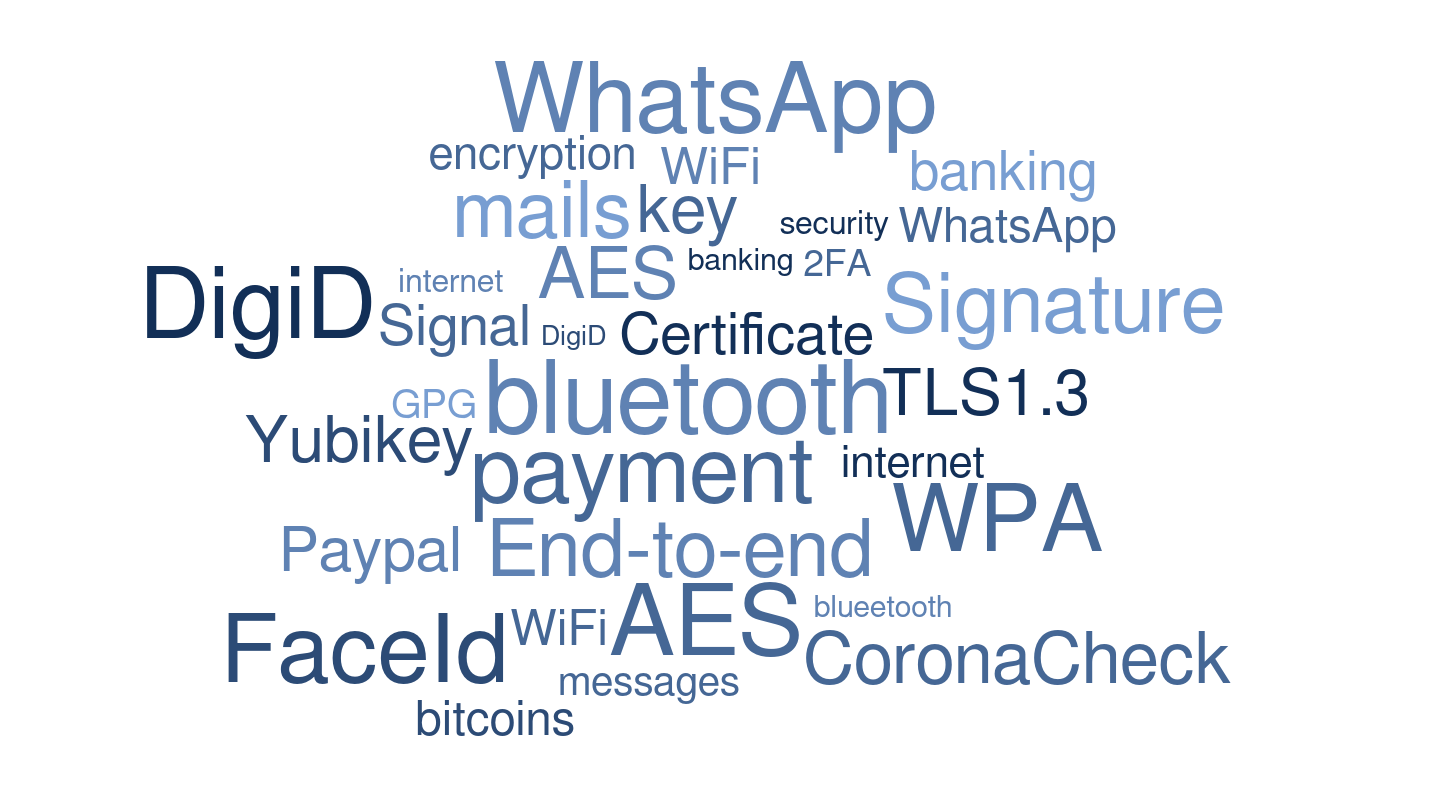
\includegraphics[width=0.85\textwidth]{graphics/everyday}
	\end{center}
\end{frame}

\begin{frame}{Crypto 101.}
	\vspace{1.25cm}
	\textbf{\large\color{PhDBlue}\underline{Symmetric encryption scheme}}
	\begin{center}
		\begin{figure}
			\begin{tikzpicture}[scale=1]

				\tikzstyle{every node}=[transform shape];
				\tikzstyle{every node}=[node distance=1.2cm];

				\begin{scope}[xshift=0cm]
					\node (f) [draw,rectangle,thick,minimum width=1.5em] {$\mathcal{E}$};
					\node (P) [left of=f,node distance=1.5cm, anchor=east] {$Plaintext$};
					\node (C) [right of=f,node distance=1.5cm, anchor=west] {$Ciphertext$};
					\path[line] (P) edge (f);
					\path[line] (f) edge (C);
					\node (k) [above=0.6cm of f] {};
					\path[line] (k) node[above] {secret $K$} edge (f);
					\node (desc) [left of=P,node distance=2cm, anchor=east] {Encryption:};
				\end{scope}

				\begin{scope}[yshift=-3cm]
					\node (f) [draw,rectangle,thick,minimum width=1.5em] {$\mathcal{D}$};
					\node (P) [left of=f,node distance=1.5cm, anchor=east] {$Plaintext$};
					\node (C) [right of=f,node distance=1.5cm, anchor=west] {$Ciphertext$};
					\path[line] (f) edge (P);
					\path[line] (C) edge (f);
					\node (k) [above=0.6cm of f] {};
					\path[line] (k) node[above] {secret $K$} edge (f);
					\node (desc) [left of=P,node distance=2cm, anchor=east] {Decryption:};
				\end{scope}
			\end{tikzpicture}
		\end{figure}
	\end{center}
\end{frame}

\begin{frame}{Crypto 101.}
	\vspace{1.25cm}
	\textbf{\large\color{PhDBlue}\underline{Hashing function}}
	\begin{center}
		\begin{figure}
			\begin{tikzpicture}[scale=1]

				\tikzstyle{every node}=[transform shape];
				\tikzstyle{every node}=[node distance=1.2cm];

				\begin{scope}[xshift=0cm] % unit was not in original code for question!
					\node (f) [draw,rectangle,thick,minimum width=1.5em] {$\mathcal{H}$};
					\node (P) [left of=f,node distance=1.5cm, anchor=east] {$Message$};
					\node (C) [right of=f,node distance=1.5cm, anchor=west] {$Digest$};
					\path[line] (P) edge (f);
					\path[line] (f) edge (C);
				\end{scope}
			\end{tikzpicture}
		\end{figure}
	\end{center}
	\vspace{1.5cm}
	\textbf{\large\color{PhDBlue}\underline{Message Authentication Code (MAC)}}
	\begin{center}
		\begin{figure}
			\begin{tikzpicture}[scale=1]

				\tikzstyle{every node}=[transform shape];
				\tikzstyle{every node}=[node distance=1.2cm];

				\begin{scope}[xshift=0cm] % unit was not in original code for question!
					\node (f) [draw,rectangle,thick,minimum width=1.5em] {$\mathcal{H}$};
					\node (P) [left of=f,node distance=1.5cm, anchor=east] {$Message$};
					\node (C) [right of=f,node distance=1.5cm, anchor=west] {$Tag$};
					\path[line] (P) edge (f);
					\path[line] (f) edge (C);
					\node (k) [above=0.6cm of f] {};
					\path[line] (k) node[above] {secret $K$} edge (f);
				\end{scope}
			\end{tikzpicture}
		\end{figure}
	\end{center}
\end{frame}


\begin{frame}{What my thesis is about.}
	\Large
	\vspace{1cm}
	\begin{columns}
		\begin{column}{0.6\textwidth}
			\vspace{1cm}

			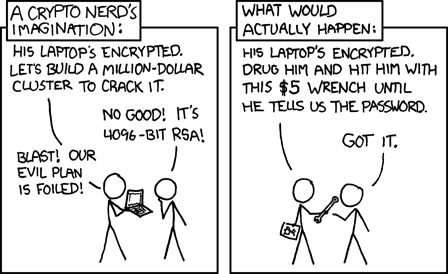
\includegraphics[width=0.9\textwidth]{graphics/security.png}
			\small
			\url{https://xkcd.com/538/}
		\end{column}
		\begin{column}{0.45\textwidth}
			\begin{itemize}
				\item Designing
				\item Implementing
				\item Breaking
				\item Verifying
				\item Standardizing
			\end{itemize}
			\vspace{0.25cm}
			\hspace{1cm} ... cryptography.
		\end{column}
	\end{columns}
\end{frame}


\framepic[0.35]{graphics/gimli}{Designing.}{
	\vspace{3.5cm}
	\Large
	\textbf{\color{PhDBlue}\underline{Gimli}}
	\vspace{0.25cm}
	\begin{itemize}
		\item Authenticated-Encryption scheme (AE)
		\item Cross-platform and Lightweight
		\item High performances \& secure
	\end{itemize}
}

\framepic[0.25]{graphics/embeded}{Implementing.}{
	\vspace{1.5cm}
	\Large
	\textbf{\color{PhDBlue}\underline{Optimized on RISC-V}}
	\vspace{0.25cm}
	\begin{itemize}
		\item Gimli
		\item Sparkle
		\item Saturnin
		\item Ascon
		\item Delirium
		\item Xoodyak
		\item AES
		\item Keccak
	\end{itemize}
}

\framepic[0.25]{graphics/magnifying_glass}{Breaking.}{
	\vspace{2.5cm}
	\Large
	\textbf{\color{PhDBlue}\underline{Cryptanalysis of Morus}}
	\renewcommand{\arraystretch}{1.5}
	\vspace{0.25cm}
	\begin{itemize}
		\item Morus is a high-performances AE scheme.
		\item[]
			\vspace{0.25cm}
			\begin{tabular}{r|c|c}
				           & complexity claim & our result        \\
				\hline
				Morus-640  & $2^{128}$        & $2^{146}$         \\
				Morus-1280 & $2^{256}$        & \emphp{$2^{152}$} \\
			\end{tabular}
	\end{itemize}
}



\framepic[0.25]{graphics/coq}{Verifying.}{
	\vspace{2cm}
	\Large
	\textbf{\color{PhDBlue}\underline{Proof of correctness of X25519 in TweetNaCl}}\\
	\vspace{0.5cm}
	Using the Coq theorem prover, we verify:
	\begin{itemize}
		\item the correctness of the C implementation,
		\item that it matches RFC 7748,
		\item and we link with X25519 maths definition.
	\end{itemize}

	\vspace{0.5cm}
	First complete proof from C to the maths definition.
}

\begin{frame}{Standardizing.}
	\vspace{2cm}
	\Large
	\begin{columns}
		\begin{column}{0.5\textwidth}
			\begin{itemize}
				\item KangarooTwelve\\
				      (SHA-3 \emph{on steroids})
				\item 1$^{st}$ Draft in January 2017,
				\item Still not accepted...
				\item CFRG is very slow.
			\end{itemize}
		\end{column}
		\begin{column}{0.5\textwidth}
			\begin{flushright}
				
\includegraphics[width=\textwidth]{graphics/standards_2x.png}\\
				\small
				\url{https://xkcd.com/927/}
			\end{flushright}
		\end{column}
	\end{columns}
\end{frame}
% \begin{frame}[fragile]
% 	\frametitle{Compiling}

% 	\begin{alertblock}{Warning}
% 		You can ignore this slide if you \textbf{are} working with Overleaf.
% 	\end{alertblock}

% 	To compile this deck you'll need the \texttt{biber} package. Probably your \TeX editor already supports it; if not, you will easily find online the instructions to install it.

% 	\vskip 0.5cm

% 	If you're not using an editor, you can compile this presentation using the command line by running:

% 	\begin{verbatim}
% $ pdflatex main.tex
% $ biber main.bcf
% $ pdflatex main.tex
% $ pdflatex main.tex
% \end{verbatim}


% \end{frame}

% \section{Colors}

% \begin{frame}{Colors}

% 	For this template we defined four colors, following the graphic profile of Umeå University:
% 	\begin{itemize}
% 		\item \textcolor{white}{\marker[PhDBlue]{\texttt{PhDBlue}}}
% 		\item \textcolor{white}{\marker[PhDGreen]{\texttt{PhDGreen}}}
% 		\item \textcolor{white}{\marker[PhDPink]{\texttt{PhDPink}}}
% 		\item \textcolor{white}{\marker[PhDGold]{\texttt{PhDGold}}}
% 	\end{itemize}

% 	\vskip 0.5cm

% 	You can use these colors as you want in your presentation. For example, you can \textbf{\textcolor{PhDGreen}{color the text in green}} by writing \texttt{\textbackslash textcolor\{PhDGreen\}\{my green text\}}.

% 	\vskip 0.5cm

% 	We also redefined many of the most common \LaTeX{} and Beamer commands, like \texttt{itemize}, \texttt{block}, etc. You will see samples of these commands in the following slides.

% \end{frame}

% \section{Blocks}
% \begin{frame}
% 	\begin{center}
% 		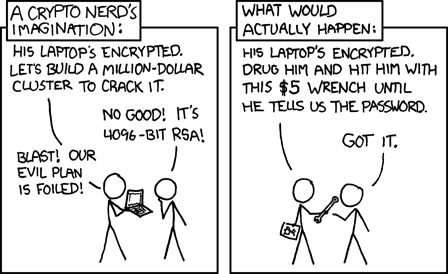
\includegraphics[width=0.7\textwidth]{graphics/security.png}
% 	\end{center}
% \end{frame}


\begin{frame}
	\begin{center}
		\vspace{1.25cm}
		\huge
		\color{PhDBlue}
		\textbf{Thank you for your attention.}

		\vspace{1cm}

		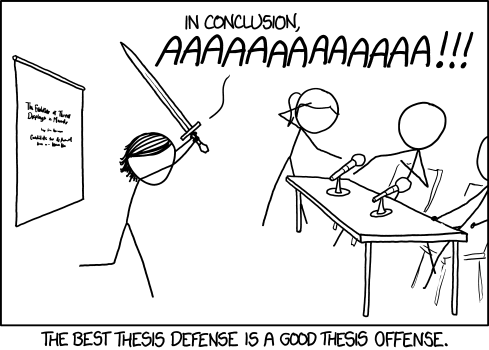
\includegraphics[width=0.5\textwidth]{graphics/thesis_defense.png}\\
		\small
		\url{https://xkcd.com/1403/}
	\end{center}
\end{frame}

% \section{Enumerates, itemizes and description}

% \subsection{Enumerates and itemizes}


% \begin{frame}{Enumerates and itemizes}

% 	This is an example of \texttt{itemize}.
% 	\begin{itemize}
% 		\item A long time ago in a galaxy far, far away...
% 	\end{itemize}
% 	And this is an example of \texttt{enumerate}.

% 	\begin{enumerate}
% 		\item Go to the Death Star.
% 		\item Find the exhaust port.
% 		\item Make the perfect shot.
% 		\item Become a hero.
% 	\end{enumerate}
% \end{frame}

% \subsection{Description}

% \begin{frame}[fragile]
% 	\frametitle{Description}
% 	This is an example of \texttt{description}.

% 	\begin{description}
% 		\item<2->[Vader] \emph{I am} your father.
% 		\item<1->[Luke] No. No! That's not true! \textbf{That's impossible!}
% 	\end{description}

% 	\begin{uncoverenv}<3>
% 		\vskip 0.5cm
% 		And while we're here, let's have a look to \texttt{verbatim} as well, to see how we made items appear in arbitrary order:
% 		\vskip 0.5cm
% 		\begin{verbatim}
% \begin{description}
%   \item<2->[This is the first item - appears after] one
%   \item<1->[This is the second item - appears first] two
% \end{description}
%   \end{verbatim}
% 	\end{uncoverenv}

% \end{frame}

% \section{Maths}

% \begin{frame}{Maths}
% 	A formula will look like this:
% 	\begin{center}
% 		$x^2 + y^2 = z^2$
% 	\end{center}

% 	You can number equations as well:
% 	\begin{equation}
% 		1+1=2
% 	\end{equation}

% 	\begin{equation}
% 		1+1=2 \tag{custom label!}
% 	\end{equation}

% 	\vskip 0.5cm

% 	If you want to use the sans serif math fonts, or use a serif font for the main text, just go to \texttt{beamerfontthemephd.sty} and select the indicated font option.

% \end{frame}

% \begin{frame}{Theorems}

% 	The usual \texttt{theorem}, \texttt{corollary}, \texttt{definition}, \texttt{definitions}, \texttt{fact}, \texttt{example} and \texttt{examples} blocks are available as well.

% 	\begin{theorem}
% 		There exists an infinite set.
% 	\end{theorem}
% 	\begin{proof}
% 		This follows from the axiom of infinity.
% 	\end{proof}
% 	\begin{example}[Natural Numbers]
% 		The set of natural numbers is infinite.
% 	\end{example}

% \end{frame}

% \section{Other blocks}

% \begin{frame}{Other blocks}

% 	Here we display examples of \texttt{abstract}, \texttt{verse}, \texttt{quotation}, and \texttt{quote}.

% 	\vskip 0.5cm

% 	\begin{abstract}
% 		This is an abstract.
% 	\end{abstract}
% 	\begin{verse}
% 		This is a verse.
% 	\end{verse}
% 	\begin{quotation}
% 		This is a quotation.

% 		\raggedleft -Han Solo
% 	\end{quotation}
% 	\begin{quote}
% 		A quote this is.

% 		\raggedleft -Yoda
% 	\end{quote}

% \end{frame}

% \section{Bibliography and Publications}
% \begin{frame}[fragile]
% 	\frametitle{Bibliography}

% 	You can cite an article
% 	\begin{itemize}
% 		\item normally using \texttt{\textbackslash cite}, e.g.: (\cite{article1})
% 		\item or display the full citation using \texttt{\textbackslash fullcite}, e.g.:  \fullcite{article1} \\\vspace{0.4cm}

% 		      \textit{(n.d.) stands for "no date". \texttt{year=\{A long time ago...\}} is not a date that should be specified in \texttt{bibliography} anyway.}
% 	\end{itemize}

% 	\vskip 0.5cm
% 	Look at the code of the following slide to see how to automatically split the bibliography on many slides. You can also use \texttt{\textbackslash nocite\{*\}} to display the non-cited publications as well.

% \end{frame}

% \begin{frame}[t,allowframebreaks]
% 	\frametitle{Bibliography}

% 	\nocite{*} % will display the non-cited publications as well. Useful for a publication list.

% 	\printbibliography

% \end{frame}

% \section{Bonus Commands}

% \begin{frame}[fragile]
% 	\frametitle{Framecard}

% 	You can display a frame with a colored background and a huge text in the center using the command \texttt{\textbackslash framecard}.
% 	\vskip 0.5cm
% 	For example, you can write:
% 	\begin{verbatim}
% \framecard{A SECTION\\TITLE}
% \end{verbatim}

% 	This will display a frame with a blue background and the phrase "A SECTION TITLE" in the center. You can also use a custom color with \texttt{\textbackslash framecard}:
% 	\begin{verbatim}
% \framecard{A SECTION\\TITLE}
% \framecard[PhDGreen]{A SECTION TITLE\\
% WITH A CUSTOM COLOR}
% \end{verbatim}
% 	You can see the results of the commands above in the following slides.

% \end{frame}

% \framecard{A SECTION \\\vspace{3pt} TITLE}
% \framecard[PhDGreen]{A SECTION TITLE\\\vspace{3pt}WITH A CUSTOM COLOR}

% \begin{frame}[fragile]
% 	\frametitle{Framepic}

% 	You can display a frame with a background image using the command \texttt{\textbackslash framepic}. The image will be \textbf{adapted vertically} to fit the the frame.

% 	For example, you can write:
% 	\begin{verbatim}
% \framepic{graphics/darth}{
% 	\framefill
%     \textcolor{white}{Luke,\\I am your supervisor}
%     \vskip 0.5cm
% }
% \end{verbatim}

% 	Alternatively, to make the background 50\% transparent, you can write \texttt{\textbackslash framepic[0.5]\{graphics/darth\}...}


% 	You can see the results of the commands above in the following slides.

% \end{frame}


% \framepic{graphics/darth}{
% 	\framefill
% 	\textcolor{white}{Luke,\\I am your supervisor}
% 	\vskip 0.5cm
% }

% \framepic[0.5]{graphics/darth}{
% 	\vfill
% 	\begin{flushright}
% 		\textcolor{PhDBlue}{\textbf{Right-aligned text with\\Semi-transparent background}}
% 	\end{flushright}
% }

% \begin{frame}[t,fragile,allowframebreaks]
% 	\frametitle{Other bonus commands}

% 	We provide two other bonus commands:
% 	\begin{description}
% 		\item[\texttt{pdfnewline}] you can use \texttt{\textbackslash pdfnewline} to avoid the annoying \texttt{hyperref} related warnings when using newlines in the document's title, author, etc. For example, in this presentation the author is defined as:
% 			\begin{verbatim}
% \author[Luke Skywalker]{
%   Luke Skywalker, Ph.D.
%   \pdfnewline
%   \texttt{luke.skywalker@phd.se}
% }
% \end{verbatim}
% 		\item[\texttt{marker}] you can use \texttt{\textbackslash marker} to highlight some text. The default color is \marker{pink}, but you can also \marker[PhDGold]{use a custom color}. For example:
% 			\begin{verbatim}
% \marker{Default color}
% \marker[PhDGold]{Custom Color}
% \end{verbatim}
% 		\item[\texttt{framefill}] you can use \texttt{\textbackslash framefill} to put the text at the bottom of a slide by filling all the vertical space.
% 	\end{description}

% \end{frame}

\end{document}